\subsection{Perceptual Hashing}
Neben der mittleren quadratischen Abweichung ist eine der einfachsten, aber auch
anfälligsten Methoden zur Bestimmung der Ähnlichkeit von zwei Bildern, das
Hashing. Dabei gibt es viele verschiedene Ansätze und Vorgehensmodelle. Die
gängigste Methode ist die Anwendung des pHashes, auch genannt Perceptual Hashing.
\parencite{hashing-apiumhub}

Beim Perceptual Hashing werden sowohl für das Referenz- als auch für Testbild
ein Hash berechnet. Die aus deren Differenz resultierende Hamming-Distanz ergibt
die Übereinstimmung der Bilder. Je geringer die Distanz, desto ähnlicher. Das
Verfahren ist nicht normiert und noch ein offenes Forschungsthema.
\parencite{hashing-phash}

Im Folgenden wird ein beispielhaftes pHash-Verfahren erläutert. Zuerst wird
sowohl das Referenz- als auch das Testbild in eine Graustufen-Grafik
umgewandelt. Schließlich wird die Grafik auf 32x32 Pixel skaliert. Auf das
entstandene Grauwertbild folgen zwei diskrete Kosinus Transformationen (1. Pro
Zeile, 2. Pro Spalte). Die hochfrequenten Abschnitte befinden sich nun links
oben in einer 8x8 Matrix. Daraufhin wird der Median-Grauwert der 64 Pixel
berechnet. Jeder Pixel, dessen Grauwert unter dem Median liegt, wird weiß
eingefärbt, der Rest schwarz. Daraus ergibt sich ein 64-Bit langer Hashwert
(schwarz: 0, weiß: 1). Abbildung \ref{fig:phash-process} verdeutlicht den 
Ablauf zur Generierung des Hashes anhand einer Testgrafik. Zuletzt wird zwischen
den beiden generierten Bitfolgen der Hamming-Abstand berechnet. Je niedriger der
Abstand der beiden Bitfolgen ist, desto größer ist die Übereinstimmung zwischen
den Eingabebildern. \parencite{hashing-apiumhub}

\begin{figure}[H]
    \centering
    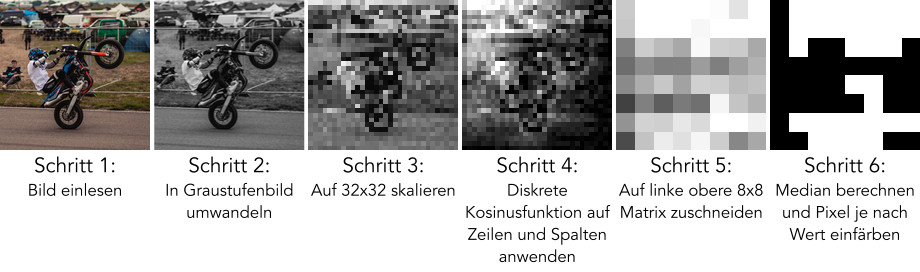
\includegraphics[width=\textwidth]{phash-process}
    \caption{PHASH: Schrittweise Berechnung des Hashes}
    \label{fig:phash-process}
    \bildquelle{Eigene Darstellung; Zugehöriger Programmcode im \hyperlink{page.14}{Anhang}}
\end{figure}

\noindent{\textbf{Vorteile}}
\begin{itemize}[topsep=0pt]
    \item Verhältnismäßig einfache Implementierung möglich
    \item Schnelle Suchperformance, wenn die Hashes der Referenzbilder bereits
    in einer dafür geeigneten Datenstruktur (z.B. k-d-Bäume, VP-Bäume,
    Kugelbäume) vorliegen \parencite{hashing-lvngd}
    \item Robust gegen Wasserzeichen, Farbfilter, leichte Helligkeits- und
    Kontraständerungen, Gammakorrekturen, Skalierungen sowie Komprimierungen
    (siehe Abbildung \ref{fig:phash})
    \parencite{hashing-phash}
\end{itemize}

\noindent{\textbf{Nachteile}}
\begin{itemize}[topsep=0pt]
    \item Nicht robust gegen Spiegelungen, Rotierungen und Verzerrungen (siehe
    Abbildung \ref{fig:phash})
    \item Nicht robust gegen Zuschneidungen, neu eingefügte Elemente oder
    Änderungen des Blickwinkels
\end{itemize}

\begin{figure}[H]
    \centering
    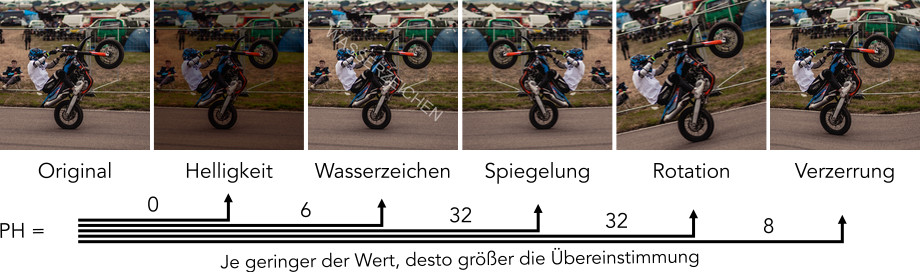
\includegraphics[width=\textwidth]{phash}
    \caption{PHASH: Anwendung an verschiedenen Testbildern}
    \label{fig:phash}
    \bildquelle{Eigene Darstellung}
\end{figure}